% Figura do Cap. I: ciclo de funcionamento de um Expert Advisor. Substitui a
% figura de Almeida (2016) em 27/10/2026, a pedido do autor. Desde 29/10/2026 é a
% alternativa E1b de ia/rascunhos/diagramas_2026-10-27/ea_v2.pdf, com as
% funções de evento do MQL5 (a E1a, sem elas, está no mesmo rascunho). Desenho
% genérico, vale para qualquer EA. Compilada pelo Makefile do tg/.
\documentclass[11pt,border=2pt]{standalone}
\usepackage[T1]{fontenc}
\usepackage[utf8]{inputenc}
\usepackage{mathptmx}
\usepackage{tikz}
\usetikzlibrary{arrows.meta,positioning,shapes.geometric,fit,backgrounds}
\tikzset{
  seta/.style={-{Stealth[length=2.2mm]}, semithick},
  caixa/.style={rectangle, draw, semithick, fill=gray!10, rounded corners=2pt,
                align=center, minimum width=58mm, minimum height=9mm, font=\small},
  decisao/.style={diamond, draw, semithick, fill=white, aspect=2.6, align=center,
                  inner sep=1pt, font=\small},
  evento/.style={rectangle, draw, semithick, fill=gray!25, rounded corners=8pt,
                 align=center, minimum width=58mm, minimum height=9mm, font=\small},
  rotulo/.style={font=\footnotesize\itshape, align=center},
  funcao/.style={font=\footnotesize\ttfamily, align=right},
}
\begin{document}
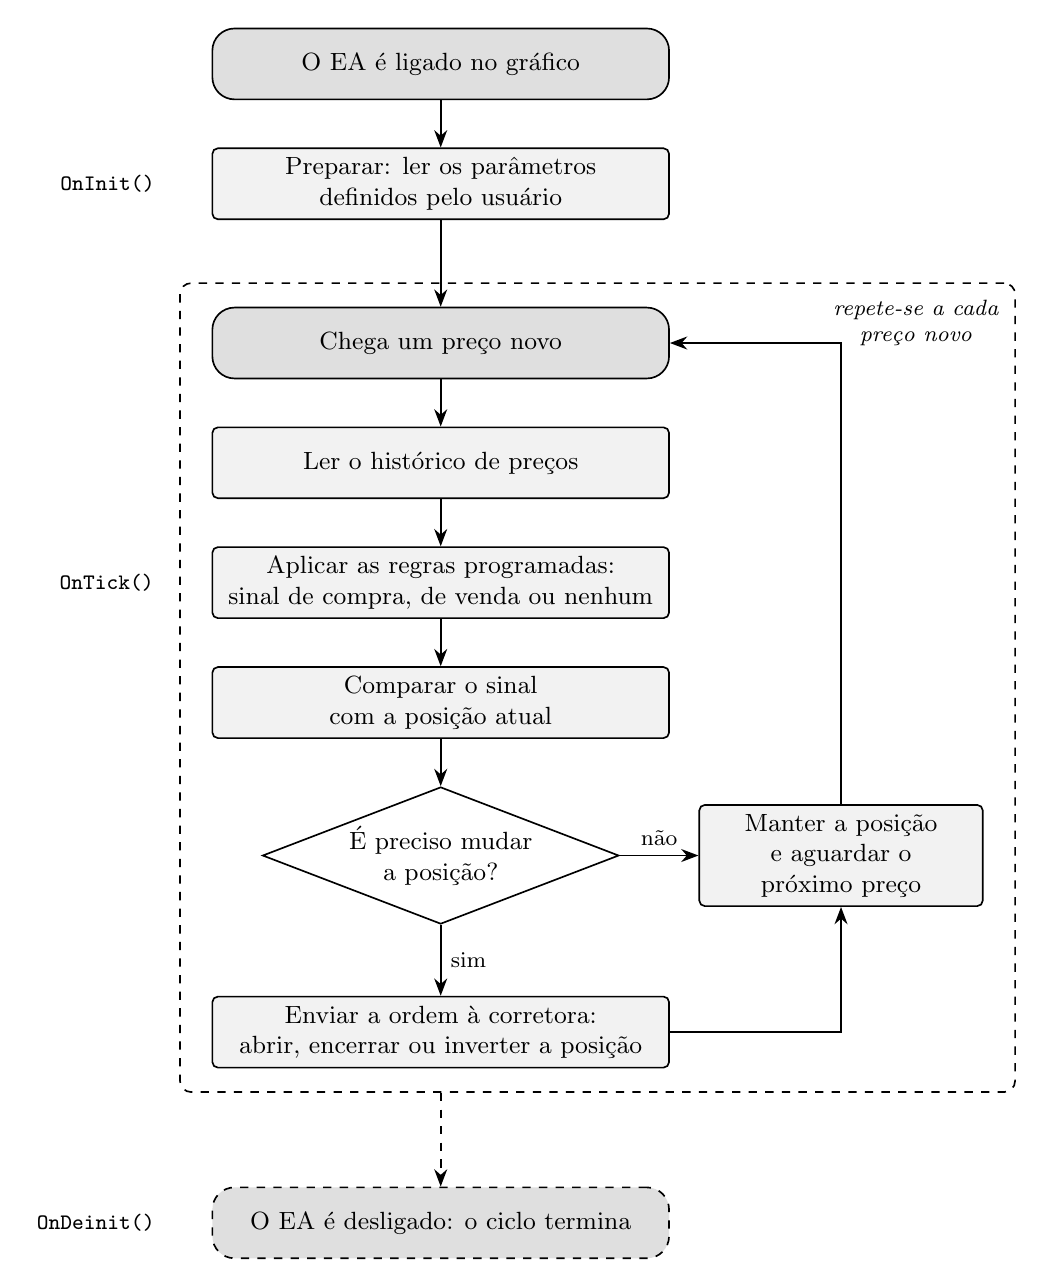
\begin{tikzpicture}[node distance=6mm]
  \node[evento] (liga) {O EA é ligado no gráfico};
  \node[caixa, below=of liga] (prep) {Preparar: ler os parâmetros\\definidos pelo usuário};
  \node[evento, below=11mm of prep] (ev) {Chega um preço novo};
  \node[caixa, below=of ev] (le) {Ler o histórico de preços};
  \node[caixa, below=of le] (ap) {Aplicar as regras programadas:\\sinal de compra, de venda ou nenhum};
  \node[caixa, below=of ap] (po) {Comparar o sinal\\com a posição atual};
  \node[decisao, below=of po] (dc) {É preciso mudar\\a posição?};
  \node[caixa, below=9mm of dc] (or) {Enviar a ordem à corretora:\\abrir, encerrar ou inverter a posição};
  \node[caixa, right=10mm of dc, minimum width=36mm] (es) {Manter a posição\\e aguardar o\\próximo preço};
  \node[evento, below=15mm of or, dashed] (fim) {O EA é desligado: o ciclo termina};

  \draw[seta] (liga) -- (prep);
  \draw[seta] (prep) -- (ev);
  \draw[seta] (ev) -- (le);
  \draw[seta] (le) -- (ap);
  \draw[seta] (ap) -- (po);
  \draw[seta] (po) -- (dc);
  \draw[seta] (dc) -- node[right, font=\footnotesize]{sim} (or);
  \draw[seta] (dc) -- node[above, font=\footnotesize]{não} (es);
  \draw[seta] (or.east) -| (es.south);
  \draw[seta] (es.north) |- (ev.east);

  \begin{scope}[on background layer]
    \node[draw, dashed, semithick, rounded corners=4pt, inner xsep=4mm, inner ysep=3mm,
          fit=(ev)(or)(es)] (ciclo) {};
  \end{scope}
  \node[rotulo, anchor=north east] at ([xshift=-1mm,yshift=-1mm]ciclo.north east)
    {repete-se a cada\\preço novo};
  \draw[seta, dashed] (ciclo.south -| fim.north) -- (fim.north);

  \node[funcao, left=6mm of prep] {OnInit()};
  \node[funcao, anchor=east] at ([xshift=-2mm]ciclo.west |- ap) {OnTick()};
  \node[funcao, left=6mm of fim] {OnDeinit()};
\end{tikzpicture}
\end{document}
